%% LyX 2.3.6.1 created this file.  For more info, see http://www.lyx.org/.
%% Do not edit unless you really know what you are doing.
\documentclass[english]{article}
\usepackage[T1]{fontenc}
\usepackage[latin9]{inputenc}
\usepackage{geometry}
\geometry{verbose,tmargin=2.5cm,bmargin=2.5cm,lmargin=2.5cm,rmargin=2.5cm}
\usepackage{array}
\usepackage{textcomp}
\usepackage{multirow}
\usepackage{amstext}
\usepackage{graphicx}

\makeatletter

%%%%%%%%%%%%%%%%%%%%%%%%%%%%%% LyX specific LaTeX commands.
\newcommand{\lyxmathsym}[1]{\ifmmode\begingroup\def\b@ld{bold}
  \text{\ifx\math@version\b@ld\bfseries\fi#1}\endgroup\else#1\fi}

%% Because html converters don't know tabularnewline
\providecommand{\tabularnewline}{\\}

\makeatother

\usepackage{babel}
\begin{document}
{[}SPLIT\_HERE{]}
\begin{enumerate}
\item \textbf{{[}ACJC/PRELIM/9569/2021/P1/Q1{]} }

A food delivery app offers promotions to customers based on their
usage pattern. 

First time customers would receive a \$5 discount on their first purchase.
If a customer has spent at least \$1000 on the app in the last 3 months,
the app would upgrade the customer to Gold status and offer 10\% discount
on all orders. 

Gold status customers who have been inactive for 1 month would be
offered an additional 5\% discount on top of the existing 10\% discount.
Customers who have made their first purchase and have been inactive
for 1 month would receive a \$5 discount instead. 
\begin{enumerate}
\item Create a decision table to show these conditions and actions. \hfill{}{[}4{]}
\item Simplify your decision table by removing redundancies from the decision
table. \hfill{}{[}1{]}
\end{enumerate}
{[}SPLIT\_HERE{]}
\item \textbf{{[}ACJC/PRELIM/9569/2021/P1/Q2{]} }

The recursive function \texttt{Binomial} has two parameters, \texttt{N}
and \texttt{R}.

\noindent %
\noindent\begin{minipage}[t]{1\columnwidth}%
\texttt{01\qquad{}FUNCTION Binomial(N, R : INTEGERS) RETURNS INTEGER }

\texttt{02\qquad{}\qquad{}IF R = 0 OR R = N }

\texttt{03\qquad{}\qquad{}\qquad{}THEN }

\texttt{04\qquad{}\qquad{}\qquad{}\qquad{}Answer \textleftarrow{}
1 }

\texttt{05\qquad{}\qquad{}\qquad{}ELSE }

\texttt{06\qquad{}\qquad{}\qquad{}\qquad{}Answer \textleftarrow{}
Binomial(N \textendash{} 1, R) + Binomial(N \textendash{} 1, R \textendash{}
1) }

\texttt{07\qquad{}\qquad{}ENDIF }

\texttt{08\qquad{}\qquad{}RETURN Answer }

\texttt{09\qquad{}ENDFUNCTION}%
\end{minipage}
\begin{enumerate}
\item State what is meant by a recursive function, and identify the line
number that makes \texttt{Binomial} recursive. \hfill{}{[}2{]}
\item An example of a trace tree diagram showing the recursive function
call \texttt{Binomial(3,1)} is shown.
\begin{center}
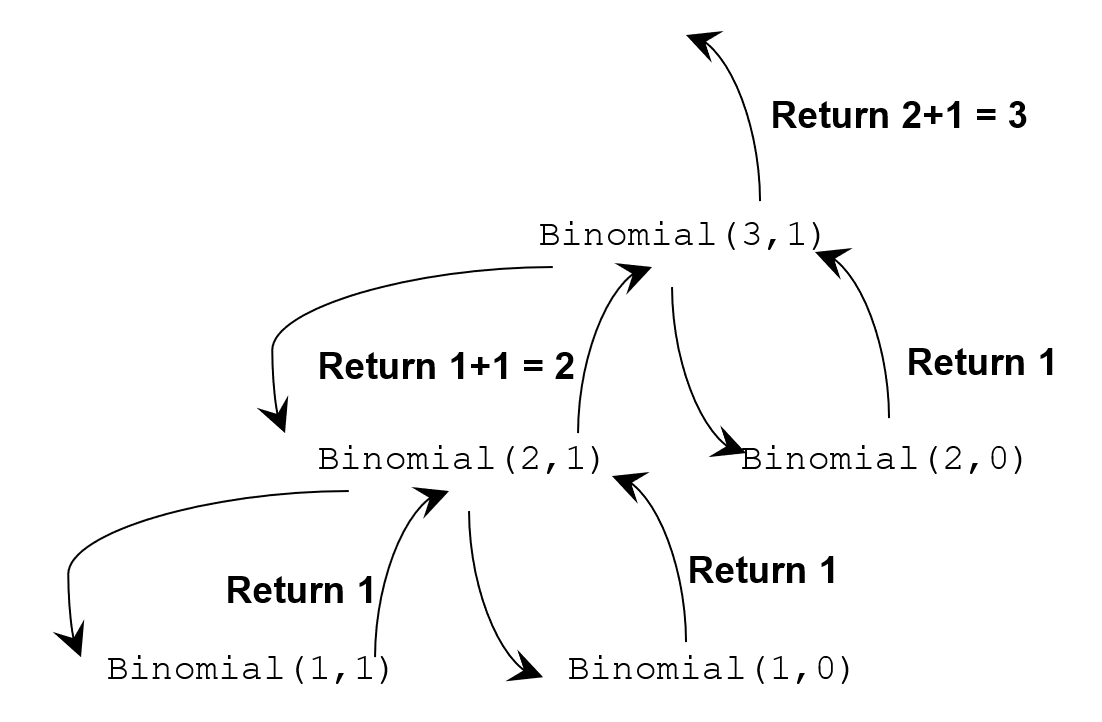
\includegraphics[width=0.5\paperwidth]{C:/Users/Admin/Desktop/Github/question_bank/LyX/static/img/9569-ACJC-2020-P1-Q2}
\par\end{center}

\end{enumerate}
Use the above example to create a trace tree diagram for the recursive
function call \texttt{Binomial(3,2)}. \hfill{}{[}4{]}
\begin{enumerate}
\item[(c)] Give values of N and R which would cause the function to enter infinite
recursion. \hfill{}{[}2{]}
\end{enumerate}
{[}SPLIT\_HERE{]}
\item \textbf{{[}ACJC/PRELIM/9569/2021/P1/Q3{]} }

The function \texttt{Evaluate} is designed to evaluate a polynomial
at a given value of $x$. The polynomial is stored as a queue of coefficients
in descending powers of x.

For example, the polynomial $5x^{3}-2x^{2}+3x-1$ is given as the
queue $[5,\lyxmathsym{\textendash}2,3,\lyxmathsym{\textendash}1]$,
where 5 is at the head of the queue.

\noindent %
\noindent\begin{minipage}[t]{1\columnwidth}%
\texttt{01\qquad{}FUNCTION Evaluate(X : INTEGER, Coeffs : QUEUE)
RETURNS INTEGER }

\texttt{02\qquad{}\qquad{}Answer \textleftarrow{} 0 }

\texttt{03\qquad{}\qquad{}REPEAT }

\texttt{04\qquad{}\qquad{}\qquad{}Answer \textleftarrow{} Answer
+ DEQUEUE Coeffs }

\texttt{05\qquad{}\qquad{}\qquad{}Answer \textleftarrow{} Answer
{*} X }

\texttt{06\qquad{}\qquad{}UNTIL Coeffs IS EMPTY }

\texttt{07\qquad{}\qquad{}RETURN Answer }

\texttt{08\qquad{}ENDFUNCTION}%
\end{minipage}
\begin{enumerate}
\item Draw a trace table to determine the output of the function \texttt{Evaluate}
for \texttt{X = 2} and \texttt{Coeffs = {[}5, \textendash 2, 3, \textendash 1{]}},
as described above. \hfill{}{[}4{]}
\item Describe the error in the function \texttt{Evaluate} as it is currently
written. \hfill{}{[}1{]}
\item Rewrite the pseudo-code above so that \texttt{Evaluate} returns the
correct value of the polynomial at a given value of \texttt{x}. \hfill{}{[}4{]}
\end{enumerate}
{[}SPLIT\_HERE{]}
\item \textbf{{[}ACJC/PRELIM/9569/2021/P1/Q4{]} }

During Home-Based Learning, many lessons were carried out over the
Internet.
\begin{enumerate}
\item For lessons carried out by video conferencing, tools by external companies
such as Zoom or Google Meet were used.

Give one example of an ethical consideration companies such as Zoom
or Google should take into account in this situation. \hfill{}{[}1{]}
\item Many lesson resources and homework submissions were carried out via
file uploads. Describe how a file can be uploaded from a student\textquoteright s
computer to a cloud drive by packet switching.\hfill{} {[}4{]}
\item For a Mother Tongue lesson, a teacher created a webpage in a non-English
language. Some students who accessed the webpage saw random characters
instead of the content intended by the teacher.
\begin{enumerate}
\item Describe the relevance of communications protocols in this context.
\hfill{}{[}2{]}
\item Describe how Unicode might address some of these problems.\hfill{}
{[}1{]}
\end{enumerate}
\end{enumerate}
{[}SPLIT\_HERE{]}
\item \textbf{{[}ACJC/PRELIM/9569/2021/P1/Q5{]} }

A printing shop offers printing services to its customers. When a
printing order is sent to the shop, the following information is recorded
down:
\begin{itemize}
\item Date of order 
\item Name of customer 
\item Number of copies 
\item Colour, or black and white, printing 
\item Whether express printing is required
\end{itemize}
The printing shop accepts three types of orders, leaflets, books and
posters.

Customers printing leaflets or books need to indicate if they require
single side or double side printing.

In addition, for books, the type of cover (hard cover or soft cover)
would need to be recorded. 

Leaflets and books are available in three sizes (A3, A4 or A5), while
posters are only available in a fixed size of A2.

For poster printing, customers have a choice of either glossy or matte
finishing.

The total charge to user is determined by the specifications of the
order and the formula is unique for each type of order.

This system is to be implemented using object-oriented programming
(OOP).
\begin{enumerate}
\item Draw a class diagram, showing:
\begin{itemize}
\item Any derived classes and inheritance from the base class 
\item The properties needed in the base, and any derived classes 
\item Suitable methods to support the system with at least one getter and
setter
\end{itemize}
The base class is \texttt{BASIC\_ORDER}. \hfill{}{[}8{]}
\item Explain the purpose of inheritance in object-oriented programing.
\hfill{}{[}2{]}
\end{enumerate}
{[}SPLIT\_HERE{]}
\item \textbf{{[}ACJC/PRELIM/9569/2021/P1/Q6{]} }

In a computer game, players\textquoteright{} names and scores are
stored in a binary search tree, in increasing order of score.

The binary search tree has its data inserted in the following order:

Ryan 18 

Bella 25 

Joshua 27 

Shane 20 

Jasmine 17 

Alexis 21 

Leslie 15
\begin{enumerate}
\item Draw the binary search tree. \hfill{}{[}4{]}
\item The binary search tree is implemented using the two dimensional array
shown below. Copy and fill in the entries in the array.
\noindent \begin{center}
\begin{tabular}{|c|c|c|c|c|}
\hline 
Index & Name & Score & Left Pointer & Right Pointer\tabularnewline
\hline 
0 &  &  &  & \tabularnewline
\hline 
1 &  &  &  & \tabularnewline
\hline 
2 &  &  &  & \tabularnewline
\hline 
3 &  &  &  & \tabularnewline
\hline 
4 &  &  &  & \tabularnewline
\hline 
5 &  &  &  & \tabularnewline
\hline 
6 &  &  &  & \tabularnewline
\hline 
\end{tabular}
\par\end{center}

\hfill{}{[}5{]}
\item To delete a node from a binary tree, the following cases are considered:
\noindent \begin{center}
\begin{tabular}{|l|l|}
\hline 
Case & Action\tabularnewline
\hline 
Node has no children & - Node is removed from tree\tabularnewline
\hline 
Node has one child & - Node is replaced with its child\tabularnewline
\hline 
\multirow{4}{*}{Node has two children} & - Call the node to be deleted $D$. Do not delete$D$\tabularnewline
\cline{2-2} 
 & - Look for the node $E$ that comes after $D$ in an in-order traversal\tabularnewline
\cline{2-2} 
 & - Copy the data $E$ into $D$.\tabularnewline
\cline{2-2} 
 & - Delete $E$ using one of the previous two cases.\tabularnewline
\hline 
\end{tabular}
\par\end{center}

Draw the tree at each step after the following players are deleted,
one after another:
\begin{enumerate}
\item Joshua \hfill{}{[}1{]}
\item Jasmine\hfill{} {[}1{]}
\item Ryan \hfill{}{[}2{]}
\end{enumerate}
\item The program has a feature which allows the user to enter an integer.
The program then returns a list of players whose score is greater
than that integer. Describe how the program can create this list using
the binary search tree. \hfill{}{[}4{]}
\end{enumerate}
{[}SPLIT\_HERE{]}

\quad{} 
\item \textbf{{[}ACJC/PRELIM/9569/2021/P1/Q7{]} }
\begin{enumerate}
\item The following is the pseudocode for an in-place quicksort algorithm
for sorting in ascending order.

\noindent %
\noindent\begin{minipage}[t]{1\columnwidth}%
\texttt{01\qquad{}FUNCTION Partition(L, R : INTEGERS, MyList : LIST)
RETURNS INTEGER }

\texttt{02\qquad{}\qquad{}Pivot \textleftarrow{} MyList{[}R{]} }

\texttt{03\qquad{}\qquad{}i \textleftarrow{} L }

\texttt{04\qquad{}\qquad{}j \textleftarrow{} L }

\texttt{05\qquad{}\qquad{}REPEAT }

\texttt{06\qquad{}\qquad{}\qquad{}IF MyList{[}j{]} > Pivot }

\texttt{07\qquad{}\qquad{}\qquad{}\qquad{}THEN }

\texttt{08\qquad{}\qquad{}\qquad{}\qquad{}\qquad{}}\texttt{\textbf{A}}\texttt{ }

\texttt{09\qquad{}\qquad{}\qquad{}\qquad{}ELSE }

\texttt{10\qquad{}\qquad{}\qquad{}\qquad{}Temp \textleftarrow{}
MyList{[}j{]} 11 MyList{[}j{]} \textleftarrow{} MyList{[}i{]} }

\texttt{12\qquad{}\qquad{}\qquad{}\qquad{}}\texttt{\textbf{B}}\texttt{ }

\texttt{13\qquad{}\qquad{}\qquad{}ENDIF }

\texttt{14\qquad{}\qquad{}UNTIL j = R }

\texttt{15\qquad{}\qquad{}MyList{[}R{]} \textleftarrow{} MyList{[}i{]}
// swap elements with index i and R }

\texttt{16\qquad{}\qquad{}MyList{[}i{]} \textleftarrow{} Pivot }

\texttt{17\qquad{}\qquad{}}\texttt{\textbf{C}}\texttt{ }

\texttt{18\qquad{}ENDFUNCTION }

\texttt{19\qquad{}PROCEDURE Quicksort(L, R : INTEGERS, MyList : LIST) }

\texttt{20\qquad{}\qquad{}IF }\texttt{\textbf{D}}\texttt{ }

\texttt{21\qquad{}\qquad{}\qquad{}THEN }

\texttt{22\qquad{}\qquad{}\qquad{}\qquad{}PivotPos = Partition(R,
L, MyList) }

\texttt{23\qquad{}\qquad{}\qquad{}\qquad{}CALL Quicksort(L, PivotPos
- 1, MyList) }

\texttt{24\qquad{}\qquad{}\qquad{}\qquad{}}\texttt{\textbf{E}}\texttt{ }

\texttt{25\qquad{}\qquad{}ENDIF }

\texttt{26\qquad{}ENDPROCEDURE}%
\end{minipage}
\begin{enumerate}
\item Write pseudo-code to replace \texttt{\textbf{A}}, \texttt{\textbf{B}},
\texttt{\textbf{C}}, \texttt{\textbf{D}} and \texttt{\textbf{E}} in
the above algorithm. \hfill{}{[}5{]}
\item State the time complexity of the algorithm in the above pseudo-code.
\hfill{} {[}1{]}
\item State and explain when the worst case scenario (for running time)
for quicksort arises in the above algorithm. \hfill{}{[}3{]}
\item Another programmer suggested insertion sort would be more efficient
during the worst case scenario in (iii).

State and explain if insertion sort is indeed more efficient in this
instance. \hfill{}{[}2{]}
\end{enumerate}
\item A program needs to store an array of names and scores in a two dimensional
array and perform the following:
\begin{itemize}
\item Output the names and scores in alphabetical order. 
\item Check for the presence of a particular name
\end{itemize}
The data to be stored in the array is as follows:

Peter 68 

Mary 70 

Kelvin 48 

Casper 44 

Luther 76
\begin{enumerate}
\item Draw a flowchart to represent a linear search algorithm that returns
the score of a particular name. \hfill{} {[}4{]}
\item Instead of storing the data in an array, it is suggested that the
names could be stored in a hash table instead. 

With reference to the requirements of the program, suggest one advantage
and one disadvantage of storing the names in a hash table instead
of an array. \hfill{} {[}2{]}
\item (iii) An array can be used to create the hash table data structure.
Describe the process of inserting the above data into a hash table.
You may assume there will be no collisions. \hfill{} {[}3{]}
\end{enumerate}
\end{enumerate}
{[}SPLIT\_HERE{]}
\item \textbf{{[}ACJC/PRELIM/9569/2021/P1/Q8{]} }

A programmer is tasked to write a program to store the examination
scores of students in the entire school. For each student, the database
would need to store the following data: name, form class, subject
class, subject, score and subject teacher.
\begin{enumerate}
\item Suggest a suitable data type for each of the following fields: 
\begin{itemize}
\item Name 
\item Class 
\item Score \hfill{}{[}2{]}
\end{itemize}
\item The programmer is considering storing this data in either a relational
or non-relational database.
\begin{enumerate}
\item State three key differences between the two types of databases. \hfill{}{[}3{]}
\item State and explain which database system the programmer should choose.
\hfill{}{[}3{]}
\end{enumerate}
\end{enumerate}
A healthcare group would like to store patient data in a relational
database. When a patient visits the clinic, the clinic will record
the following information:
\begin{itemize}
\item Date and time of visit 
\item Name of attending doctor and his NRIC 
\item Patient name and NRIC number
\end{itemize}
After the doctor has attended to the patient, the patient would be
given a prescription. The prescription would record the medication
which the patient is supposed to take. Each prescription, which consists
of at least one medicine, would have its own unique identification
number. Each medicine would have a unique identification number, name
and price. 

The data is stored in a relational database with five tables: \texttt{Patient},
\texttt{Doctor}, \texttt{Appointment}, \texttt{Prescription} and \texttt{Medicine}.
\begin{enumerate}
\item[(c)]  Draw the Entity-Relationship (E-R) diagram to show the tables in
third normal form (3NF) and the relationships between them. \hfill{}{[}7{]}
\item[(d)]  A table description can be written as:

\texttt{TableName (Attribute1, Attribute2, Attribute3, \dots )}

The primary key is indicated by underlining one or more attributes.
Foreign keys are indicated by using a dashed underline.

Using the information provided, write table descriptions for the tables
you identified in part (c). \hfill{}{[}8{]}
\end{enumerate}
{[}SPLIT\_HERE{]}
\item \textbf{{[}ACJC/PRELIM/9569/2021/P2/Q1{]} }

A programmer is writing a program to implement a role-playing computer
game using Object-Oriented Programming (OOP).

The players have to collect food items. A food item has the following
attributes:
\begin{itemize}
\item \texttt{name : STRING }
\item \texttt{value : INTEGER}
\end{itemize}
and the following methods:
\begin{itemize}
\item \texttt{get\_name() }
\item \texttt{get\_value()}
\end{itemize}
A player takes on the role of a person. A person has the following
attributes:
\begin{itemize}
\item \texttt{name : STRING }
\item \texttt{health : INTEGER} which is initialised at a value of \texttt{100}
\item \texttt{strength : INTEGER} which is initialised at a value of \texttt{100}
\end{itemize}
and the following methods:
\begin{itemize}
\item \texttt{get\_name() }
\item \texttt{get\_health() }
\item \texttt{get\_strength() }
\item \texttt{eat(food)} adds the value of the food to the strength. The
code should display the player\textquoteright s new strength. 
\item \texttt{attack(opponent)}
\end{itemize}
For the \texttt{attack} method, \texttt{opponent} is another person.
\begin{itemize}
\item A random integer \texttt{r} between \texttt{1} and \texttt{10} (inclusive)
is generated. 
\item If the player\textquoteright s \texttt{strength} is less than \texttt{r},
then the player does not have enough strength to attack and there
is no change to \texttt{opponent}\textquoteright s \texttt{health}. 
\item If the player\textquoteright s \texttt{strength} is at least \texttt{r},
then the attack is successful and \texttt{opponent}\textquoteright s
\texttt{health} is decreased by \texttt{r}. 
\begin{itemize}
\item If opponent\textquoteright s health is now negative, then opponent
has been defeated. 
\end{itemize}
\item The player\textquoteright s \texttt{strength} is decreased by r.
\end{itemize}
There are two subclasses of the \texttt{Person} class -- \texttt{Healer}
and the \texttt{Warrior}.

Healer has one additional method:
\begin{itemize}
\item \texttt{heal(patient)}
\end{itemize}
\quad{}

For the \texttt{heal} method, \texttt{patient} is another person.
\begin{itemize}
\item A random integer \texttt{r} between \texttt{1} and \texttt{10} (inclusive)
is generated. 
\item If the player\textquoteright s \texttt{strength} is less than \texttt{r},
then the player does not have enough strength to heal and there is
no change to \texttt{patient}\textquoteright s \texttt{health}. 
\item If the player\textquoteright s \texttt{strength} is at least \texttt{r},
then the healing is successful and \texttt{patient}\textquoteright s
\texttt{health} is increased by \texttt{r}, up to a maximum of \texttt{100}.
\end{itemize}
\texttt{Warrior}\textquoteright s \texttt{attack} method is twice
as effective, meaning that if the player has enough strength to attack,
\texttt{opponent}\textquoteright s \texttt{health} is decreased by
\texttt{2{*}r}, while the player\textquoteright s \texttt{strength}
is decreased by \texttt{r}.

\subsubsection*{Task 1.1}

Write program code to define the class \texttt{Food}. \hfill{}{[}3{]}

\subsubsection*{Task 1.2}

Write program code to define the class \texttt{Person}.

The code should display appropriate messages about the outcome of
\texttt{attack}, including the new value of opponent\textquoteright s
\texttt{health}. \hfill{}{[}10{]}

\subsubsection*{Task 1.3}

Use appropriate inheritance to write program code to define the class
\texttt{Healer}.

The code should display appropriate messages about the outcome of
\texttt{heal}, including the new value of \texttt{patient}\textquoteright s
\texttt{health}. \hfill{}{[}4{]}

\subsubsection*{Task 1.4}

Use appropriate inheritance and polymorphism to write program code
to define the class \texttt{Warrior}. \hfill{}{[}2{]}

Test your code with the following steps in order:
\begin{itemize}
\item Create a \texttt{Food} item with name \texttt{'Cheese'} and value
\texttt{10}. 
\item Create a \texttt{Warrior} with \texttt{name} \texttt{'Sam'}. 
\item Create a \texttt{Healer} with name \texttt{'Alex'}. 
\item Create a \texttt{Person} with name \texttt{'Jan'}. 
\item \texttt{'Jan'} attacks \texttt{'Sam'}. 
\item \texttt{'Sam'} attacks \texttt{'Jan'}. 
\item \texttt{'Alex'} heals \texttt{'Jan'}. 
\item \texttt{'Sam'} eats \texttt{'Cheese'}.
\end{itemize}
Download your program code and output for Task 1 as \texttt{TASK1\_<your
name>\_<centre number>\_<index number>.ipynb} \hfill{}{[}3{]}

{[}SPLIT\_HERE{]}
\item \textbf{{[}ACJC/PRELIM/9569/2021/P2/Q2{]} }

An $\mathtt{n\times n}$ chessboard consists of an $\mathtt{n\times n}$
grid of small squares. For this task, the squares are numbered using
a coordinate system as a tuple of two integers. The first integer
is the column number, starting from \texttt{1} at the left, and the
second integer is the row number, starting from \texttt{1} at the
bottom.

A chess knight is a piece that occupies a square, and can then move
to another square according to one of the following rules:
\begin{itemize}
\item moving two squares horizontally and then one square vertically in
either direction, or 
\item moving two squares vertically and then one square horizontally in
either direction.
\end{itemize}
See the diagram below for examples.
\begin{center}
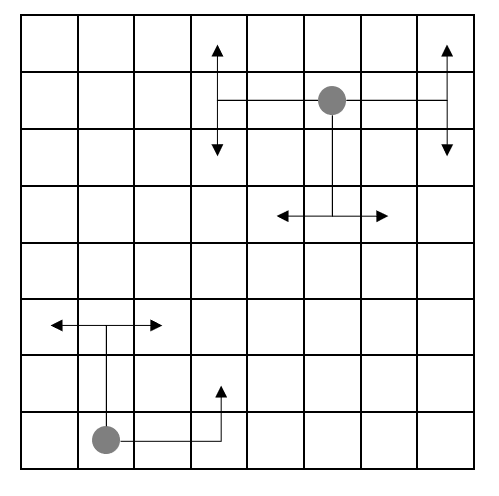
\includegraphics[width=0.5\paperwidth]{C:/Users/Admin/Desktop/Github/question_bank/LyX/static/img/9569-ACJC-2020-P2-Q2}
\par\end{center}

The knight at \texttt{(2,1)} can move to \texttt{(1,3)}, \texttt{(3,3)}
or \texttt{(4,2)}. 

The knight at \texttt{(6,7)} can move to \texttt{(4,6)}, \texttt{(4,8)},
\texttt{(5,5)}, \texttt{(7,5)}, \texttt{(8,6)} or \texttt{(8,8)}.

Only the starting and ending squares of the knight\textquoteright s
move are counted as being visited by the knight, and not the squares
that the knight passes over while moving.

A knight\textquoteright s tour is a sequence of moves that a chess
knight makes on a chessboard, so that it visits every square of the
chessboard exactly once. It does not need to return to its starting
square.

\subsubsection*{Task 2.1}

For a given value of \texttt{n} and a list of squares, write program
code to determine if the list is a knight\textquoteright s tour of
an $\mathtt{n\times n}$ chessboard.

Test your code using the values\texttt{ $\mathtt{n=7}$} and the list
of squares given in the files: 
\begin{itemize}
\item \texttt{TASK2TOUR.txt}, which is a valid tour; 
\item \texttt{TASK2NOTOUR.txt}, which is not a valid tour. \hfill{}{[}10{]}
\end{itemize}
An algorithm to generate a knight\textquoteright s tour needs to keep
track of the squares already visited, so that the knight does not
visit them a second time during the tour.

\subsubsection*{Task 2.2}

Suppose the knight is currently on square square, and a list of squares
already visited by the knight is given in \texttt{lis}.

Write a function \texttt{available(square,lis)} that returns a list
of squares which the knight can visit on its next move from \texttt{square},
and are not currently in \texttt{lis}. These are the squares available
to the knight as it tries to complete the tour.

The output should be given in lexicographic order, that is, with the
column numbers in ascending order, and, among the squares with the
same column number, with the row numbers in ascending order. \hfill{}{[}6{]}

\subsubsection*{Task 2.3}

The knight starts at \texttt{(1,1)}, the bottom left square, of an
$8\mathtt{\times}8$ chessboard.

From each square, the knight moves to the available square from which
it has the smallest number of available squares after that. If there
is a tie, the square which comes first in lexicographic order is chosen.

Write program code to generate the knight\textquoteright s tour as
a list of squares in the order they are visited.

Download your program code and output for Task 2 as \texttt{TASK2\_<your
name>\_<centre number>\_<index number>.ipynb}\hfill{} {[}9{]}

{[}SPLIT\_HERE{]}
\item \textbf{{[}ACJC/PRELIM/9569/2021/P2/Q3{]} }

A text file \texttt{INVENTORY.txt} contains the inventory data for
a certain electronics store. Each line in the file contains tab-delimited
data that shows the product name, product type, purchase price, selling
price and quantity available.

Each line is in the format

\texttt{Name\textbackslash tType\textbackslash tPurchase\_Price\textbackslash tSelling\_Price\textbackslash tQuantity}

where \texttt{\textbackslash t} represents the tab character.

\subsection*{Task 3.1 }

Write program code to:
\begin{itemize}
\item Read the inventory data from the text file; 
\item Find the average selling price of products belonging to the \texttt{Laptop}
product type and display this value; 
\item Count the number of products in each product type and store it in
appropriate data structure called \texttt{TypeCount}; 
\item Display the product type with the greatest number of products. If
there is a tie, display all of the product types with the greatest
number of products.
\end{itemize}
Download your program code and output for Task 3.1 as 

\texttt{TASK3\_1\_<your name>\_<centre number>\_<index number>.ipynb}
\hfill{}{[}6{]}

\subsection*{Task 3.2 }

The profit margin of each product can be calculated by the following
equation:
\noindent \begin{center}
Profit margin = selling price -- purchase price.
\par\end{center}

Write program code to:
\begin{itemize}
\item Calculate and display the total profit the store could make if all
products are sold; 
\item Sort the inventory data using a Merge sort algorithm in descending
order of profit margin; 
\item Display the sorted inventory data in the format given below.
\noindent \begin{center}
\texttt{}%
\begin{tabular}{lll}
\texttt{Product } & \texttt{Product Type } & \texttt{Profit Margin }\tabularnewline
\texttt{ThinkingPad 14} & \texttt{Computer } & \texttt{300 }\tabularnewline
\texttt{Bapple 8 } & \texttt{Phone } & \texttt{450}\tabularnewline
\end{tabular}
\par\end{center}

\end{itemize}
Download your program code and output for Task 3.2 as 

\texttt{TASK3\_2\_<your name>\_<centre number>\_<index number>.ipynb}\hfill{}
{[}9{]}

\subsection*{Task 3.3}

A store manager decided to make some changes to \texttt{INVENTORY.txt}
and saved it as \texttt{INVENTORY\_SERIAL.txt}. Each line in the updated
file contains tab-delimited data that shows the serial number, product
name, product type, purchase price, selling price and quantity available.

Each line is in the format:

\texttt{Serial\_No\textbackslash tName\textbackslash tType\textbackslash tPurchase\_Price\textbackslash tSelling\_Price\textbackslash tQuantity}

where \texttt{\textbackslash t} represents the tab character.

Write program code to insert the data from \texttt{INVENTORY\_SERIAL.txt}
into a NoSQL database \texttt{OUTLETS} under the collection \texttt{GEM}.

Download your program code for Task 3.3 as 

\texttt{TASK3\_3\_<your name>\_<centre number>\_<index number>.py}
\hfill{}{[}5{]}

\subsection*{Task 3.4}

The database administrator wants to validate that the store manager
did not make any errors when he edited the text file. Write program
code to check that the database conforms to the below specifications:
\begin{itemize}
\item \texttt{Serial\_No} consists of one digit followed by two letters,
followed by one digit (e.g. \texttt{1AB7}); 
\item \texttt{Name} consists of only letters, digits and spaces; 
\item \texttt{Quantity} is a positive integer. 
\end{itemize}
Any document that has an error should be removed from the database.
You may assume data fields not specified above are error free. Display
the documents that were removed.

Download your program code for Task 3.4 as 

\texttt{TASK3\_4\_<your name>\_<centre number>\_<index number>.py}
\hfill{}{[}5{]}

{[}SPLIT\_HERE{]}
\item \textbf{{[}ACJC/PRELIM/9569/2021/P2/Q4{]} }

A company keeps records of the employees working for it. The following
are the information stored in the company\textquoteright s database:
\begin{itemize}
\item \texttt{Employee\_name} -- name of the employee 
\item \texttt{Employee\_ID} -- unique ID number allocated to each employee 
\item \texttt{Job\_type} -- type of job the employee is employed for (\texttt{'Sales'}
or \texttt{'Tech\_support}') 
\item \texttt{Date\_of\_employment} -- date the employee joined the company 
\item \texttt{Service\_status} -- whether the employee is still in service
(\texttt{'True'} means the employee is still in the company, \texttt{'False'}
means the employee has left the company) 
\end{itemize}
For sales employees, the following extra information is recorded:
\begin{itemize}
\item \texttt{Total\_sales} -- the amount of sales in dollars made by the
employee 
\end{itemize}
For tech support employees, the following extra information is recorded:
\begin{itemize}
\item \texttt{Bugs\_resolved} -- the total number of bugs the employee
has resolved 
\end{itemize}
The database is expected to be normalised and stored in three different
tables:

\texttt{Employee }

\texttt{Sales }

\texttt{Tech\_support}

\subsection*{Task 4.1}

Create an SQL file called \texttt{TASK4\_1\_<your name>\_<centre number>\_<index
number>.sql} to show the SQL code to create the database \texttt{records.db}
with the three tables. Primary keys and foreign keys should be defined
where appropriate.

Save your SQL code as 

\texttt{TASK4\_1\_<your name>\_<centre number>\_<index number>.sql}
\hfill{}{[}5{]}

\subsection*{Task 4.2 }

The files \texttt{SALES.txt} and \texttt{TECH\_SUPPORT.txt} contain
information regarding the sales and tech support employees respectively.
The information should be inserted into the database.

For \texttt{SALES.txt}, information is given in the following order: 

\texttt{Employee\_ID}, \texttt{Employee\_name}, \texttt{Date\_of\_Employment},
\texttt{Service\_status}, \texttt{Total\_Sales}

For \texttt{TECH\_SUPPORT.txt}, information is given in the following
order: 

\texttt{Employee\_ID}, \texttt{Employee\_name}, \texttt{Date\_of\_Employment},
\texttt{Service\_status}, \texttt{Bugs\_resolved}

Write a python program to insert all information from the two files
into the \texttt{records} database, \texttt{records.db}. Run the program.

Save your program code as 

\texttt{TASK4\_2\_<your name>\_<centre number>\_<index number>.py}\hfill{}
{[}5{]}

\subsection*{Task 4.3}

The company wants to filter the employees by \texttt{Service\_status}
and display the results in a web browser.

Write a Python program and the necessary files to create a web application
that:
\begin{itemize}
\item receives a \texttt{Service\_status} string from a HTML form, then
\item creates and returns a HTML document that enables the web browser to
display either
\begin{itemize}
\item an ordered list of employees that are still in service, or 
\item an ordered list of employees that are no longer in service,
\end{itemize}
depending on the \texttt{Service\_status} string entered by the user.
\end{itemize}
The list should be sorted in alphabetical order.

Save your Python program as 

\texttt{TASK4\_3\_<your name>\_<centre number>\_<index number>.py }

with any additional files / sub-folders as needed in a folder named 

\texttt{TASK4\_3\_<your name>\_<centre number>\_<index number>}

Run the web application. Save the output of the program when \texttt{'TRUE'}
is entered as the \texttt{Service\_status} as \texttt{TASK4\_3\_<your
name>\_<centre number>\_<index number>.html}. \hfill{}{[}12{]}

{[}SPLIT\_HERE{]}
\end{enumerate}

\end{document}
